\documentclass[11pt,a4paper]{article}
\usepackage[margin=2.4cm]{geometry}
\usepackage{amsmath,amssymb}
\usepackage[T1]{fontenc}
\usepackage{graphicx}
\usepackage{booktabs}
\usepackage[round,authoryear]{natbib}
\usepackage{siunitx}
\usepackage[colorlinks=true,linkcolor=blue,citecolor=blue,urlcolor=blue]{hyperref}
\sisetup{range-phrase=--,range-units=single}
\graphicspath{{../../manuscript/figures_redo/}}

\title{Average number of hydrogen ionizations per primary particle:\\
photons and electrons in the neutral IGM}
\author{Response note --- \texttt{Notebooks/redo/stage8\_*}}
\date{2026--09--07}

\begin{document}
\maketitle

\begin{abstract}
\noindent
We compute $N_{\rm ion}(E,z_i)$, the average total number of H\,\textsc{i}
ionizations produced by one primary particle of energy $E$ injected at
redshift $z_i$ into the fiducial neutral IGM, counting every ionization
produced anywhere down the cascade until the end of the reionization window
($z=5.5$). Two primary species are treated: electrons (existing calculation,
\texttt{stage2\_cascade.py}) and photons (new, \texttt{stage8\_photon\_yield.py},
photoionization $+$ Compton scattering only, by request). The result is
Fig.~\ref{fig:main}. Electrons obey the familiar $W\simeq\SI{36.6(23)}{\electronvolt}$
plateau between \SI{100}{\electronvolt} and \SI{30}{\kilo\electronvolt};
photons do not, because above $\sim\SI{2.3}{\kilo\electronvolt}$ the IGM
becomes optically thin and most primaries leave the window without
interacting.
\end{abstract}

%======================================================================
\section{Assumptions}
%======================================================================

Every assumption is stated where it enters; the ones that are global are
collected here.

\paragraph{A1 --- Background and gas.}
Flat $\Lambda$CDM with the \emph{Planck} 2018 TT,TE,EE$+$lowE$+$lensing
parameters \citep{planck18}, as implemented in
\texttt{astropy.cosmology.Planck18}. The neutral hydrogen density is the
fiducial normalisation of the parent manuscript,
\begin{equation}
  n_{\rm H\,I}(z) = \SI{1.8e3}{\per\cubic\metre}
  \left(\frac{1+z}{21}\right)^{3},
  \label{eq:nHI}
\end{equation}
with a residual ionized fraction $x_e = 10^{-4}$ (free electrons enter only
as Compton targets and as the $f_{\rm free}$ branch below). Helium, clumping,
and any inhomogeneity are neglected: the medium is uniform at the mean
density. The hydrogen ionization threshold is $B_{\rm H}=\SI{13.6057}{\electronvolt}$.

\paragraph{A2 --- Window.}
Ionizations are counted only while $z > z_{\rm final} = 5.5$; a particle that
survives to $z_{\rm final}$ contributes nothing further. A second variant
extends the count to $z>3.0$ and is tabulated alongside (columns
\texttt{Nt}/\texttt{Ypt}); it changes the photon yield by
$\lesssim 6.5\%$ except in the transparency window near
\SI{10}{\kilo\electronvolt}, where it is $+58\%$ (Sect.~\ref{sec:result}).

\paragraph{A3 --- Photon interaction channels.}
\emph{By explicit instruction}, the photon cascade includes
\textbf{photoionization of H(1s) and Compton scattering only}. Pair production
on hydrogen nuclei (Bethe--Heitler) and on the CMB (Breit--Wheeler) are
\textbf{omitted}. Both omitted channels can only \emph{add} ionizations, so
the photon curve is a \textbf{lower bound} wherever they matter; the two
energies at which they switch on are computed in
Sect.~\ref{sec:verif} and marked on Fig.~\ref{fig:main}.

\paragraph{A4 --- Cross sections.}
Photoionization: the H(1s) cross section of \citet{karzas61}, normalised to
$\sigma_{\rm pi}(B_{\rm H}) = \SI{6.30e-22}{\metre\squared}$. Compton: the
free-electron Klein--Nishina cross section \citep{klein29}, both total and
differential (Eq.~\ref{eq:kn}). Regime of validity: the free-electron
(impulse) treatment of scattering off a \emph{bound} electron requires
$T \gg B_{\rm H}$; Sect.~\ref{sec:verif}\,D shows this is harmless here.

\paragraph{A5 --- Bound versus free targets.}
Per hydrogen nucleus there are $1+x_e$ electrons available for Compton
scattering, a fraction $f_{\rm bound} = 1/(1+x_e)$ bound and
$f_{\rm free} = x_e/(1+x_e)$ free. A Compton recoil $T$ on a bound electron
is itself one ionization and ejects an electron of kinetic energy $T-B_{\rm H}$
when $T \ge B_{\rm H}$, and ionizes nothing when $T<B_{\rm H}$. On a free
electron it ionizes nothing directly and simply hands over an electron of
energy $T$.

\paragraph{A6 --- Straight-line, light-speed photon transport.}
Photons travel on the null geodesic and redshift as $E \propto (1+z)$;
Compton deflection is not tracked (the medium is uniform, so only the
\emph{time} spent, not the direction, matters for the interaction budget).

\paragraph{A7 --- Electron child yields.}
The number of ionizations produced by a secondary electron of kinetic energy
$K$ released at redshift $z$ is taken from the existing table
\texttt{redo\_\allowbreak cascade\_\allowbreak table.npz},
column $Y+Y_{p}^{\rm (e)}$: the
in-situ collisional cascade plus the ionizations made by the photons
(bremsstrahlung, inverse Compton) that the electron itself radiates and that
are re-absorbed inside the window. The underlying loss processes are inverse
Compton and bremsstrahlung \citep{blumenthal70}, Coulomb losses
\citep{gould72}, collisional excitation \citep{stone02} and RBEB collisional
ionization \citep{kim00}. Two inherited caveats:
\begin{itemize}\itemsep2pt
  \item radiated photons are transported only up to
  $E_\gamma^{\rm max}=\SI{3e4}{\electronvolt}$ (above that the
  \emph{photoionization} probability is $<10^{-3}$ everywhere in the window).
  Compton absorption of those photons is not included in the electron table,
  so the electron curve is itself a mild lower bound above
  $K\sim\SI{7e8}{\electronvolt}$, where inverse-Compton photons exceed
  \SI{3e4}{\electronvolt}. This is the origin of the electron plateau at
  $N_{\rm ion}\simeq4.1\times10^{6}$ in Fig.~\ref{fig:main}a.
  \item the child-yield lookup is clipped to $z\ge7$, as in
  \texttt{stage2\_cascade.py}: a sub-keV electron thermalises in
  $\Delta z \ll 1$, and the clipping costs $0.04\%$.
\end{itemize}

\paragraph{A8 --- What is \emph{not} assumed.}
No Monte Carlo, no continuous-slowing-down shortcut for the photon, and no
iteration: the photon equation is solved exactly (Sect.~\ref{sec:deriv}).

%======================================================================
\section{Derivation}\label{sec:deriv}
%======================================================================

\subsection{Klein--Nishina in the scattered-energy fraction}

Write $a \equiv E/m_ec^2$ and $s \equiv E'/E$ for the fraction of the photon
energy that survives the scattering. The Compton relation
$E'/E = [1+a(1-\cos\theta)]^{-1}$ inverts to
$\cos\theta = 1-(1/s-1)/a$ and gives $\mathrm{d}\cos\theta = \mathrm{d}s/(a s^2)$.
Substituting into the Klein--Nishina differential cross section
\citep[][Eq.~7.5]{klein29,rl79},
$\mathrm{d}\sigma/\mathrm{d}\cos\theta = \pi r_e^2 s^2 (s + 1/s - 1 + \cos^2\theta)$,
\begin{equation}
  \frac{\mathrm{d}\sigma}{\mathrm{d}s}
  = \frac{\pi r_e^{2}}{a}\left[\,s + \frac{1}{s} - 1 + \cos^{2}\theta\,\right],
  \qquad
  \frac{1}{1+2a} \le s \le 1 ,
  \label{eq:kn}
\end{equation}
with recoil $T = E(1-s)$, so that $E = E' + T$ identically. Equation~(\ref{eq:kn})
integrates back to the standard total cross section; this is verified
symbolically in Sect.~\ref{sec:verif}\,A.

\subsection{First-interaction weights along the light path}

A photon injected at $z_i$ with energy $E$ has, at redshift $z<z_i$ along its
path, energy $E(z) = E(1+z)/(1+z_i)$ and interaction rates
\begin{equation}
  k_{\rm pi}(z) = n_{\rm H\,I}(z)\,\sigma_{\rm pi}\!\big(E(z)\big)\,c ,
  \qquad
  k_{\rm C}(z) = n_{\rm H\,I}(z)\,(1+x_e)\,\sigma_{\rm KN}\!\big(E(z)\big)\,c .
\end{equation}
With $\tau(t)=\int k_{\rm tot}\,\mathrm{d}t'$, the probability that the
\emph{first} interaction is of type $j$ and occurs in $\mathrm{d}t$ is
\begin{equation}
  \mathrm{d}P_j = k_j(t)\,e^{-\tau(t)}\,\mathrm{d}t .
  \label{eq:firstint}
\end{equation}
The path is discretised in $\ln(1+z)$ on $N_{\rm path}=192$ nodes; on each
segment $\tau$ is taken linear in $t$ and $e^{-\tau}$ is integrated
\emph{analytically}, which makes every quadrature weight non-negative and
guarantees $\sum_j\sum_{\rm path} w_j = 1-e^{-\tau_{\rm tot}}$ exactly
(Sect.~\ref{sec:verif}\,C). The branching between the two channels is
$w_{\rm pi} = w\,k_{\rm pi}/k_{\rm tot}$, $w_{\rm C} = w\,k_{\rm C}/k_{\rm tot}$.

\subsection{The cascade equation and how it is solved}

Let $N(E,z_i)$ be the quantity asked for. Collecting
Eqs.~(\ref{eq:kn})--(\ref{eq:firstint}) and A5,
\begin{align}
  N(E,z_i) =\;& \sum_{\rm path} w_{\rm pi}\,
     \Big[\,1 + Y_e\big(E(z)-B_{\rm H},\,z\big)\Big] \nonumber\\
  &+ \sum_{\rm path} w_{\rm C}
     \int_{1/(1+2a)}^{1}\! \mathrm{d}s\;p(s\,|\,E(z))
     \Big\{ f_{\rm bound}\,\Theta(T-B_{\rm H})
            \big[1 + Y_e(T-B_{\rm H},z)\big] \nonumber\\
  &\hspace{4.6cm}
          + f_{\rm free}\,Y_e(T,z)
          + N\big(E(z)\,s,\,z\big) \Big\},
  \label{eq:master}
\end{align}
where $p(s|E)$ is Eq.~(\ref{eq:kn}) normalised to unity, $T=E(z)(1-s)$, and
$Y_e$ is the electron child yield of A7. The three terms on the second and
third lines are, in order: ionization of a bound target plus the cascade of
the ejected electron; the cascade of a Compton-heated free electron; and the
\emph{continuation of the scattered photon}, which is what makes
Eq.~(\ref{eq:master}) an integral equation.

Equation~(\ref{eq:master}) is a Volterra equation in $E$: every argument on
the right-hand side is $\le E$, with equality only in the joint limit
$z\to z_i$, $s\to1$. It is therefore solved by marching \emph{upward} in
energy on a logarithmic grid of $120$ nodes spanning
\SIrange{13.6}{1e13}{\electronvolt}, exactly as \texttt{stage2\_cascade.py}
marches upward in $K$. The near-elastic Compton limit ($E\ll m_ec^2$, where
the whole scattered-photon weight falls inside one grid cell) is handled
without iteration: the bilinear interpolation weight that lands on the
current energy node is kept on the left-hand side, so each energy node
reduces to one exact linear system over the $N_z=22$ redshift rows,
\begin{equation}
  (\mathsf{I}-\mathsf{M})\,\vec{N}_{\!\cdot,i} = \vec{A} ,
\end{equation}
solved by \texttt{numpy.linalg.solve}. No relaxation, no convergence
criterion: the multiple-scattering chain is resummed exactly. The matrix is
extremely well conditioned because the \emph{absolute} first-interaction
Compton weight never exceeds $0.151$ anywhere on the grid (it is bounded by
the total interaction probability, not by the branching ratio).

The $s$-integral uses a $64$-node Gauss--Legendre rule in $u=\ln s$: the
integrand of Eq.~(\ref{eq:kn}) has a $1/s$ tail spanning up to seven decades
at $E=\SI{5}{\tera\electronvolt}$, which is flat in $u$, while for $a\ll1$
the interval shrinks as $2a$ and the rule remains exact.

%======================================================================
\section{Verification and cross-checks}\label{sec:verif}
%======================================================================

Full output: \texttt{Notebooks/redo/stage8\_verify.log}. All checks pass.

\paragraph{A --- Klein--Nishina, differential $\to$ total.}
\emph{(i) Symbolic.} \texttt{sympy} integrates Eq.~(\ref{eq:kn}) over
$s\in[1/(1+2a),1]$ for symbolic $a>0$; the difference from the closed-form
total cross section \texttt{simplify}s to exactly $0$, with numeric residuals
$\le 2\times10^{-124}$ at $a=10^{-3},0.1,1,10,10^{3}$.
\emph{(ii) Independent quadrature.} \texttt{mpmath} adaptive quadrature at
30 digits reproduces the closed form to $1.2\times10^{-16}$ relative at every
energy from \SI{1}{\electronvolt} to \SI{1e13}{\electronvolt}.
\emph{(iii) The rule actually used.} The $64$-node Gauss--Legendre rule in
$\ln s$ agrees with the closed form to $4.4\times10^{-7}$ relative, worst
case, over \SIrange{13.6}{1e13}{\electronvolt}.
\emph{(iv) Thomson limit.} The quadrature reproduces the low-energy expansion
$\sigma_{\rm KN}/\sigma_{\rm T} = 1-2a+\tfrac{26}{5}a^2-\tfrac{133}{10}a^3$
\citep[][\S22]{heitler54} to all displayed digits.
\emph{Flagged:} the float64 evaluation of the closed-form
$\sigma_{\rm KN}$ in \texttt{redo\_common.py} loses $4\times10^{-7}$ relative
accuracy at \SI{10}{\electronvolt} and $10^{-5}$ at \SI{1}{\electronvolt} to
cancellation. This is far below every other error here and is recorded, not
fixed.

\paragraph{B --- Compton kinematics.}
All quadrature nodes lie inside $[1/(1+2a),1]$; the analytic endpoint
$s_{\min}=1/(1+2a)$ and $T_{\max}=E\,2a/(1+2a)$ are reproduced;
$E=E'+T$ holds identically by construction.

\paragraph{C --- Path kernel.}
At every $(z_i,E)$ tested, all weights are non-negative and
$\sum w = 1-e^{-\tau_{\rm tot}}$ to better than $0.5\%$ against an
independent $4\times$-finer trapezoidal evaluation of $\tau_{\rm tot}$
(typically to $10^{-5}$ relative).

\paragraph{D --- Channel competition and the impulse approximation.}
$\sigma_{\rm pi}=\sigma_{\rm C}$ at
$E=\SI{2.333}{\kilo\electronvolt}$. The maximum Compton recoil
$T_{\max}=E\,2a/(1+2a)$ reaches $B_{\rm H}$ only at
$E=\SI{1.871}{\kilo\electronvolt}$. Below that energy \emph{every} Compton
event is sub-threshold: the model produces no ionization and returns the
photon with $E'\simeq E$, which is what bound-electron (Rayleigh/Raman)
scattering does as well, so the free-electron treatment cannot bias the
ionization budget there. Above it, $T\gg B_{\rm H}$ within a factor of a few
and the impulse approximation is the standard one
\citep{zdziarski89}. Photoionization dominates the total interaction rate all
the way to \SI{2.3}{\kilo\electronvolt}, so Compton never controls the yield
below $\sim\SI{2}{\kilo\electronvolt}$.

\paragraph{E --- Omitted channel I: Bethe--Heitler pair production on H.}
Using the high-energy no-screening formula
$\sigma = 4\alpha r_e^2 Z(Z+1)[\tfrac79\ln 2k - \tfrac{109}{54}]$ and the
complete-screening formula
$\sigma = 4\alpha r_e^2 Z(Z+1)[\tfrac79\ln(183Z^{-1/3}) - \tfrac{1}{54}]$
\citep[][\S26]{heitler54,motz69}, with $Z=1$ and $Z\to Z(Z+1)=2$ for triplet
production, the complete-screening asymptote is
$\sigma_{\rm pair}=\SI{1.87e-30}{\metre\squared}$ and
$\sigma_{\rm pair}=\sigma_{\rm KN}$ at
\begin{equation}
  E_{\rm pair} = 54 \pm \SI{17}{\mega\electronvolt}
  \qquad\text{(the two screening limits bracket the true crossing).}
\end{equation}
Above the conservative edge \SI{37}{\mega\electronvolt} the photon curve is a
lower bound.

\paragraph{F --- Omitted channel II: pair production on the CMB.}
Integrating the Breit--Wheeler cross section
\citep{breit34}\citep[][\S11-3]{jauch76} over the full Planck spectrum at
$T_{\rm CMB}=2.7255(1+z)\,$K, and requiring the mean free path (evaluated at
the injection redshift, where the CMB is hottest and the onset earliest) to
fall below the proper light path down to $z=5.5$, gives
\begin{center}
\begin{tabular}{lcc}
\toprule
$z_i$ & light path [m] & $E_{\gamma\gamma}$ [eV] \\
\midrule
20 & $8.14\times10^{24}$ & $2.44\times10^{12}$ \\
15 & $7.29\times10^{24}$ & $3.33\times10^{12}$ \\
10 & $5.36\times10^{24}$ & $5.25\times10^{12}$ \\
 7 & $2.63\times10^{24}$ & $7.87\times10^{12}$ \\
\bottomrule
\end{tabular}
\end{center}
so the top decade of the grid is also a lower bound. (The naive threshold
against a typical CMB photon, $(m_ec^2)^2/kT$, is \SI{53}{\tera\electronvolt}
at $z=20$; the Wien tail brings the onset down by a factor $\sim20$.)

\paragraph{G --- Numerical convergence.}
The complete march was repeated with every discretisation doubled:
$N_{\rm path}\!: 192\to384$, $N_s\!: 64\to128$, energy nodes $120\to239$.
Both tables are interpolated log--log to the same energies (comparing nearest
grid nodes would report the grid offset, not the error). The largest change
anywhere in $7\le z_i\le20$, \SIrange{20}{1e12}{\electronvolt} is
\textbf{1.7\%}, at $E=\SI{10}{\kilo\electronvolt}$, $z_i=10$ --- the
transparency minimum, where the curve has its sharpest curvature in $\ln E$
and the interpolation itself dominates the difference. Outside the
\SIrange{0.5}{10}{\kilo\electronvolt} transparency band the change is below
$\mathbf{0.5\%}$ everywhere, and below $2\times10^{-5}$ above
\SI{1}{\giga\electronvolt}. \textbf{We therefore quote a numerical
uncertainty of $0.5\%$ on the tabulated yields, rising to $2\%$ in the
\SIrange{0.5}{10}{\kilo\electronvolt} band.}

\paragraph{H --- Physical limits (independent check of the full march).}
Where the IGM is optically thick the answer is known in closed form: the
photon is certainly photoionized, giving one ionization plus the cascade of a
photoelectron of energy $E-B_{\rm H}$, i.e.
$N_\gamma(E) = 1 + Y_e(E-B_{\rm H})$ exactly. The march, which knows nothing
of this shortcut, reproduces it:
\begin{center}
\begin{tabular}{lccccc}
\toprule
$E$ [eV] & 20.4 & 90.6 & 297 & 478 & 975 \\
\midrule
$N_\gamma / [1+Y_e(E-B_{\rm H})]$, $z_i=20$
 & $1.0000$ & $0.9999$ & $0.9968$ & $0.9835$ & $0.878$ \\
$N_\gamma / [1+Y_e(E-B_{\rm H})]$, $z_i=10$
 & $1.0000$ & $0.9998$ & $0.9916$ & $0.9602$ & $0.688$ \\
\bottomrule
\end{tabular}
\end{center}
The agreement is exact to four digits wherever
$P_{\rm int}=1$, and departs only as the photon starts to survive to
$z_{\rm final}$ ($P_{\rm int}=0.856$ at \SI{975}{\electronvolt} for $z_i=10$),
which is the physically correct behaviour. At threshold the table gives
$N=0.99989$ at \SI{13.61}{\electronvolt} and $N=1.00000$ at
\SI{20.4}{\electronvolt}, as it must.

%======================================================================
\section{Final result}\label{sec:result}
%======================================================================

\begin{figure}[htbp]
  \centering
  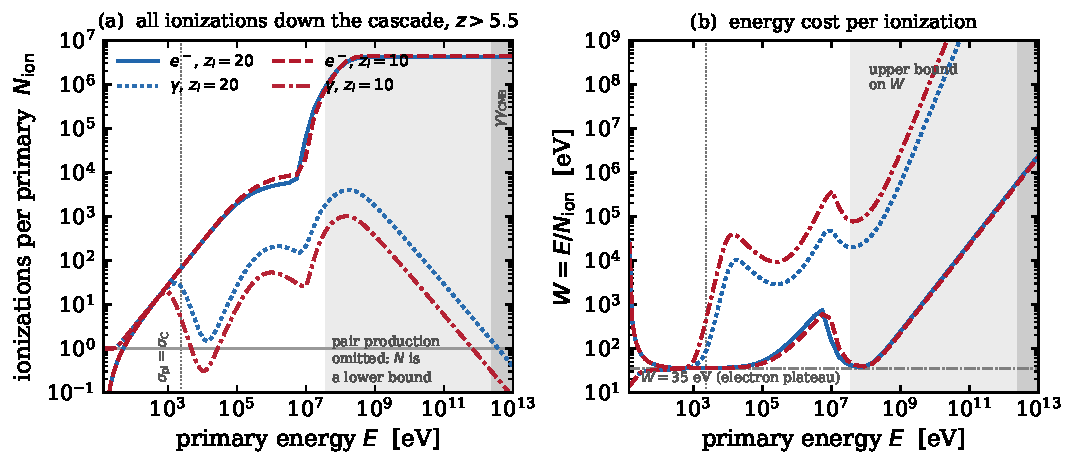
\includegraphics[width=\textwidth]{fig_ionizations_per_primary.pdf}
  \caption{Average number of hydrogen ionizations produced by one primary
  particle of energy $E$ injected at $z_i$, counting all ionizations down the
  cascade until $z=5.5$. Solid/dashed: electrons ($z_i=20$, $z_i=10$);
  dotted/dash-dotted: photons. Vertical dotted line:
  $\sigma_{\rm pi}=\sigma_{\rm C}$ at \SI{2.33}{\kilo\electronvolt}. Light
  shading: pair production on H omitted, so $N$ is a lower bound
  ($E>\SI{37}{\mega\electronvolt}$). Dark shading: pair production on the CMB
  also omitted ($E>\SI{2.4}{\tera\electronvolt}$ at $z_i=20$).
  (b) The same as the energy cost per ionization $W=E/N_{\rm ion}$; the
  dash-dotted grey line is the canonical \SI{35}{\electronvolt}.}
  \label{fig:main}
\end{figure}

\begin{table}[htbp]
\centering
\caption{$N_{\rm ion}$ per primary particle. Numerical uncertainty is the
convergence bound of Sect.~\ref{sec:verif}\,G; the systematic uncertainty
from the omitted photon channels is one-sided (the true value is larger) and
is indicated by the shading in Fig.~\ref{fig:main}.}
\label{tab:main}
\begin{tabular}{lcccc}
\toprule
& \multicolumn{2}{c}{electron} & \multicolumn{2}{c}{photon} \\
\cmidrule(lr){2-3}\cmidrule(lr){4-5}
$E$ [eV] & $z_i=20$ & $z_i=10$ & $z_i=20$ & $z_i=10$ \\
\midrule
$10^{2}$  & $2.66$              & $2.66$              & $2.81$              & $2.81$ \\
$10^{3}$  & $28.3$              & $28.3$              & $24.8$              & $19.5$ \\
$10^{4}$  & $323$               & $326$               & $1.65$              & $0.303$ \\
$10^{5}$  & $2.09\times10^{3}$  & $2.36\times10^{3}$  & $22.8$              & $7.24$ \\
$10^{6}$  & $4.88\times10^{3}$  & $6.76\times10^{3}$  & $198$               & $53.7$ \\
$10^{7}$  & $5.53\times10^{4}$  & $1.94\times10^{4}$  & $226$               & $27.8$ \\
$10^{8}$  & $2.24\times10^{6}$  & $2.22\times10^{6}$  & $3.75\times10^{3}$  & $981$ \\
$10^{10}$ & $4.14\times10^{6}$  & $4.46\times10^{6}$  & $231$               & $46.7$ \\
$10^{12}$ & $4.14\times10^{6}$  & $4.46\times10^{6}$  & $3.63$              & $0.726$ \\
\bottomrule
\end{tabular}
\end{table}

\subsection*{Reading of the figure}

\paragraph{Electrons.}
$W = K/N_{\rm ion}$ is flat at
$\SI{36.6(23)}{\electronvolt}$ (min $35.38$, max $40.03$, mean $36.63$ over
\SIrange{100}{3e4}{\electronvolt} at $z_i=20$; $36.55$ eV at $z_i=10$), the
standard result for a cascade in a nearly neutral medium
\citep{shull85,furlanetto10}. Above $\sim\SI{30}{\kilo\electronvolt}$ the
electron range starts to exceed the window and $W$ climbs; the sharp rise of
$N_{\rm ion}$ between \SIrange{1e7}{1e9}{\electronvolt} is the onset of
inverse-Compton emission into the absorbable band ($E_\gamma\lesssim
\SI{3e4}{\electronvolt}$), and the plateau at $4.1\times10^{6}$ above
\SI{1e9}{\electronvolt} is the point where the IC photons leave that band
(A7).

\paragraph{Photons.}
Three regimes:
\begin{enumerate}\itemsep2pt
  \item \SIrange{13.6}{500}{\electronvolt}: the IGM is optically thick to
  photoionization, $P_{\rm int}=1$, and the photon behaves \emph{exactly} like
  one ionization plus an electron of energy $E-B_{\rm H}$
  (Sect.~\ref{sec:verif}\,H). Because of that extra ionization the photon
  curve sits slightly \emph{above} the electron curve at the same energy
  (by $27\%$ at \SI{90}{\electronvolt}, $7\%$ at \SI{300}{\electronvolt}),
  the two merging as $E$ grows. Between \SIrange{500}{2300}{\electronvolt} the
  photon starts to survive the window and the curves separate downward.
  \item \SIrange{2.3}{100}{\kilo\electronvolt}: the transparency window.
  $\sigma_{\rm pi}\propto E^{-3}$ collapses, and the total interaction
  probability at $z_i=20$ falls from $1$ at \SI{2}{\kilo\electronvolt} to
  $0.157$ at \SI{10}{\kilo\electronvolt}. $N_{\rm ion}$ has a sharp minimum,
  $N=1.45$ at \SI{13.3}{\kilo\electronvolt} ($z_i=20$) and $N=0.303$ at
  \SI{10.5}{\kilo\electronvolt} ($z_i=10$): \emph{a \SI{10}{\kilo\electronvolt}
  photon injected at $z=10$ produces, on average, less than one ionization
  before the end of reionization.} This is the single most important feature
  of the figure and the qualitative difference from the electron case.
  \item $>\SI{100}{\kilo\electronvolt}$: Compton takes over. The interaction
  probability keeps falling ($6.4\times10^{-2}$ at \SI{1}{\mega\electronvolt},
  $2.8\times10^{-3}$ at \SI{100}{\mega\electronvolt}, $5.4\times10^{-5}$ at
  \SI{10}{\giga\electronvolt} for $z_i=20$) but the yield \emph{per}
  interaction grows faster, because the Compton recoil approaches $E$ and the
  resulting electron is itself an efficient ioniser. The product peaks at
  $N\simeq3.9\times10^{3}$ near \SI{1.4e8}{\electronvolt} and then declines as
  $N\propto E^{-1}$ once the electron yield saturates.
\end{enumerate}

\paragraph{Window sensitivity (A2).}
Extending the count from $z>5.5$ to $z>3.0$ changes the photon yield at
$z_i=20$ by $+0.0\%$ (\SI{1}{\kilo\electronvolt}), $+1.9\%$
(\SI{89}{\kilo\electronvolt}), $+6.5\%$ (\SI{1}{\mega\electronvolt}) and
$+4.9\%$ (\SI{100}{\mega\electronvolt}) --- but by $+58\%$ at
\SI{10.5}{\kilo\electronvolt}, precisely in the transparency window, where the
result is dominated by how long the photon is allowed to keep travelling.
Quoted photon yields near \SI{10}{\kilo\electronvolt} are therefore
window-definition dependent at the tens-of-per-cent level; everywhere else
they are not.


%======================================================================
\section{Why UV photons, not energetic particles, reionize the Universe}
\label{sec:why}
%======================================================================

Figure~\ref{fig:main}a is easily misread as saying that electrons are the more
effective ionizing agents, since a \SI{1}{\giga\electronvolt} electron makes
$4\times10^{6}$ ionizations and no photon on the grid makes more than
$4\times10^{3}$. That reading confuses two different questions. The figure is
\emph{per primary particle}; reionization is decided by
\begin{equation}
  \mathcal{N}_{\rm ion}
  \;=\;
  \underbrace{\frac{1}{W(E)}}_{\text{ionizations per erg}}
  \;\times\;
  \underbrace{\mathcal{E}_{\rm channel}}_{\text{ergs available}} ,
  \label{eq:budget}
\end{equation}
and \emph{both} factors favour the ultraviolet. Panel (b) of
Fig.~\ref{fig:main} already contains the first factor; the second is source
physics and is taken from the literature. The combination is
Fig.~\ref{fig:budget}, computed by \texttt{stage9\_budget.py}.

\subsection{Assumptions of this section}

The inputs are listed with their provenance; none is invented.
\begin{center}
\footnotesize
\begin{tabular}{p{1.7cm}p{3.5cm}p{4.5cm}p{4.6cm}}
\toprule
symbol & value & meaning & source \\
\midrule
$\xi_{\rm ion}$ & $10^{25.2}\,{\rm Hz\,erg^{-1}}$ & ionizing photon prod.\ eff.
  & \citet{robertson15,bouwens16} \\
$L_\nu^{\rm UV}/{\rm SFR}$ & $(1.15\times10^{-28})^{-1}$ \newline erg\,s$^{-1}$Hz$^{-1}$ per $M_\odot$yr$^{-1}$ & UV luminosity per SFR
  & \citet{kennicutt98,madau14} \\
$\langle E_\gamma\rangle$ & 20 eV & mean ionizing photon energy
  & Pop II population, 18--25 eV \\
$f_{\rm esc}$ & $0.1$ & UV escape fraction
  & \citet{robertson15,finkelstein19} \\
$L_X/{\rm SFR}$ & $3\times10^{39}$--$10^{40}$ \newline erg\,s$^{-1}$ per $M_\odot$yr$^{-1}$
  & HMXB X-rays, 0.5--8 keV
  & \citet{mineo12,fragos13,lehmer21} \\
$\Gamma_X$ & $2$ & HMXB photon index & \citet{fragos13} \\
$\mathcal{E}_{\rm CR}/M_\ast$ & $1.4\times10^{48}\,{\rm erg}\,M_\odot^{-1}$
  & all cosmic rays, \emph{measured}
  & \citet{strong10}\,/\,\citet{licquia15} \\
$\mathcal{E}_{{\rm CR}e}/M_\ast$ & $2.1\times10^{46}\,{\rm erg}\,M_\odot^{-1}$
  \newline (range $1.5$--$2.9\times10^{46}$)
  & CR \emph{electrons}, \emph{measured}
  & \citet{strong10}\,/\,\citet{licquia15} \\
$K_{ep}$ & $0.012$--$0.021$ (measured) & CR electron/proton injected-power
  ratio & \citet{strong10}, Table 2 \\
\midrule
\multicolumn{4}{l}{\emph{cross-check chain for the two CR rows, recomputed in
  \texttt{stage9\_verify\_budget.py}}} \\
$E_{\rm SN}$ & $10^{51}$ erg per CCSN & canonical explosion energy
  & \citet{woosley95} \\
$M_\ast/N_{\rm CCSN}$ & $84.8\,M_\odot$ (Chabrier) \newline $135\,M_\odot$ (Salpeter)
  & recomputed from the IMF here, $8$--$100\,M_\odot$ progenitors
  & \citet{chabrier03,salpeter55} \\
$\varepsilon_{\rm CR}$ & $0.1$ (range 0.1--0.5) & SN shock kinetic energy
  $\to$ cosmic rays
  & \citet{drury89,caprioli14}, via \citet{gesseyjones23} \\
\bottomrule
\end{tabular}
\end{center}
Uncertainties on these are factors of a few, not orders of magnitude, except
$L_X/{\rm SFR}$ and $\varepsilon_{\rm CR}$, which are scanned explicitly below.
Everything is normalised per solar mass of star formation, so the comparison is
independent of the star formation history.

\subsection{First factor: the optimum is at threshold, not at high energy}

Table~\ref{tab:pererg} reads $1/W$ off the stage 8 tables at $z_i=10$.

\begin{table}[htbp]
\centering
\caption{Ionizations per erg of injected energy, from
Fig.~\ref{fig:main}b. The last column is normalised to a
\SI{20}{\electronvolt} UV photon.}
\label{tab:pererg}
\begin{tabular}{lccc}
\toprule
channel & $W$ [eV] & ionizations erg$^{-1}$ & relative \\
\midrule
UV photon, \SI{20}{\electronvolt}        & $20.4$              & $3.06\times10^{10}$ & $1.000$ \\
UV photon, \SI{30}{\electronvolt}        & $28.5$              & $2.19\times10^{10}$ & $0.717$ \\
soft X-ray, \SI{0.5}{\kilo\electronvolt} & $35.7$              & $1.75\times10^{10}$ & $0.572$ \\
X-ray, \SI{1}{\kilo\electronvolt}        & $52.5$              & $1.19\times10^{10}$ & $0.389$ \\
X-ray, \SI{3}{\kilo\electronvolt}        & $1.08\times10^{3}$  & $5.80\times10^{8}$  & $0.019$ \\
hard X-ray, \SI{10}{\kilo\electronvolt}  & $3.21\times10^{4}$  & $1.95\times10^{7}$  & $6.4\times10^{-4}$ \\
\midrule
electron, \SI{1}{\kilo\electronvolt}     & $35.4$              & $1.77\times10^{10}$ & $0.577$ \\
electron, \SI{1}{\mega\electronvolt}     & $149$               & $4.20\times10^{9}$  & $0.137$ \\
CR electron, \SI{1}{\giga\electronvolt}  & $225$               & $2.77\times10^{9}$  & $0.091$ \\
CR electron, \SI{1}{\tera\electronvolt}  & $2.24\times10^{5}$  & $2.78\times10^{6}$  & $9.1\times10^{-5}$ \\
\midrule
HMXB power law, $\Gamma=2$, \SIrange{0.5}{8}{\kilo\electronvolt}
  & $110$ & $5.68\times10^{9}$ & $0.186$ \\
\bottomrule
\end{tabular}
\end{table}

Three statements follow, all of them visible in Fig.~\ref{fig:main}b and none
of them obvious from Fig.~\ref{fig:main}a.

\paragraph{(i) A threshold photon is the perfect ioniser.}
A photon of \SI{13.6}{\electronvolt} deposits \emph{all} of its energy in one
ionization, $W = B_{\rm H}$, which is the thermodynamic optimum: no agent can
do better. Our own table gives $N=1.00000$ at \SI{20.4}{\electronvolt}. A fast
electron cannot reach it, because it spends roughly a third of its energy on
collisional excitation (Ly$\alpha$) and a third on Coulomb heating for every
third spent on ionization \citep{shull85,valdes08,furlanetto10}; hence the
familiar $W\simeq\SI{35}{\electronvolt}$ floor rather than
\SI{13.6}{\electronvolt}. \emph{Per erg, UV photons beat the best possible
electron by a factor $\simeq2$.}

\paragraph{(ii) Above \SI{2}{\kilo\electronvolt} the IGM stops absorbing.}
This is the transparency window found in Sect.~\ref{sec:result}: the
bound--free cross section falls as $\sigma_{\rm pi}\propto E^{-3}$, the
crossover to Compton occurs at \SI{2.33}{\kilo\electronvolt}
(Sect.~\ref{sec:verif}\,D), and the total interaction probability inside the
window collapses from $1$ at \SI{2}{\kilo\electronvolt} to $0.157$ at
\SI{10}{\kilo\electronvolt} ($z_i=20$). This is the standard statement that
hard X-rays have a mean free path comparable to the Hubble scale
\citep{oh01,venkatesan01,mcquinn12,mesinger13}: they do not fail to ionize
\emph{efficiently}, they fail to interact \emph{at all} within the window. The
consequence in Table~\ref{tab:pererg} is a factor $1.6\times10^{3}$ penalty
between \SI{0.5}{\kilo\electronvolt} and \SI{10}{\kilo\electronvolt}.

\paragraph{(iii) High-energy electrons are also inefficient per erg.}
A \SI{1}{\giga\electronvolt} electron makes $4\times10^{6}$ ionizations, but it
costs \SI{1}{\giga\electronvolt} to make: $W=\SI{225}{\electronvolt}$, an order
of magnitude worse than UV. The reason is visible in
Fig.~\ref{fig:main}b: above $\sim\SI{1}{\mega\electronvolt}$ the electron cools
predominantly by inverse Compton scattering on the CMB, and most of the
up-scattered photons land above \SI{3e4}{\electronvolt}, i.e.\ inside the
transparency window of (ii), and leave. So the two failure modes are the same
failure mode.

\subsection{Second factor: the energy budgets differ by three to four orders of
magnitude}

\begin{table}[htbp]
\centering
\caption{Energy available per solar mass of star formation, and the
ionizations it delivers when multiplied by Table~\ref{tab:pererg}.
Note the deliberate asymmetry in $f_{\rm esc}$ (see text).}
\label{tab:budget}
\begin{tabular}{lccc}
\toprule
channel & erg $M_\odot^{-1}$ & $N_{\rm ion}$ $M_\odot^{-1}$ & relative to UV \\
\midrule
stellar H-ionizing UV (intrinsic)      & $1.39\times10^{50}$ & --- & --- \\
\quad escaping, $f_{\rm esc}=0.1$      & $1.39\times10^{49}$ & $4.26\times10^{59}$ & $1$ \\
HMXB X-rays, $L_X/{\rm SFR}=3\times10^{39}$ & $9.5\times10^{46}$ & $5.4\times10^{56}$ & $1.3\times10^{-3}$ \\
HMXB X-rays, $L_X/{\rm SFR}=10^{40}$   & $3.2\times10^{47}$ & $1.8\times10^{57}$ & $4.2\times10^{-3}$ \\
cosmic rays, all species               & $1.44\times10^{48}$ & $\sim4.0\times10^{57}$$^{\dagger}$ & $\sim9.4\times10^{-3}$$^{\dagger}$ \\
cosmic-ray \emph{electrons}            & $2.1\times10^{46}$ & $5.7\times10^{55}$ & $1.3\times10^{-4}$ \\
\quad range from the MW anchor         & $1.5$--$2.9\times10^{46}$ & --- & $(1.0$--$1.9)\times10^{-4}$ \\
\bottomrule
\end{tabular}\\[2pt]
{\footnotesize $^{\dagger}$ \textbf{Low confidence, flagged.} No proton cascade
was computed in this project. The entry assumes a proton $W$ comparable to the
electron one and is indicative only; the published limit is ``no more than a
few per cent'' \citep{sazonov15,leite17}, with which it agrees.}
\end{table}

The intrinsic UV budget is $1.4\times10^{50}\,{\rm erg}\,M_\odot^{-1}$
($4.3\times10^{60}$ ionizing photons per $M_\odot$, i.e.\
$\log_{10}N_{\rm ion}/M_\odot = 60.64$, the standard value). Even after the
$f_{\rm esc}=0.1$ penalty it exceeds the HMXB X-ray budget by $\sim40$--$150$
and the cosmic-ray \emph{electron} budget by $1.4\times10^{3}$.

Two points deserve emphasis because they are the ones usually left implicit.

\paragraph{The escape asymmetry is real and it is the hard channels' only
advantage.} The UV number carries $f_{\rm esc}\simeq0.1$ while the X-ray and
cosmic-ray numbers carry $f_{\rm esc}\simeq1$: the same $E^{-3}$ cross section
that makes the IGM transparent to X-rays makes the \emph{host galaxy}
transparent to them as well. That asymmetry is worth a factor $\sim10$ to the
hard channels and is precisely why they are discussed at all
\citep{oh01,mcquinn12}. It is still not nearly enough.

\paragraph{Where the cosmic-ray electron budget comes from
($2.1\times10^{46}\,{\rm erg}\,M_\odot^{-1}$).}
This number is \emph{measured}, not assembled from assumptions.
\citet{strong10} fit the GALPROP propagation model to direct cosmic-ray
measurements, non-thermal radio, hard X-ray and $\gamma$-ray data, and report
in their Table~2 the \emph{injected} cosmic-ray luminosity of the Milky Way
split by species over six propagation models: $6.6$--$8.1\times10^{40}\,
{\rm erg\,s^{-1}}$ in total (headline value $7.9\times10^{40}$),
$6.0$--$7.4\times10^{40}$ in protons and
$8.65\times10^{38}$--$1.34\times10^{39}\,{\rm erg\,s^{-1}}$ in
\emph{primary electrons}. Dividing by the Milky Way star formation rate,
${\rm SFR}=1.65\pm0.19\,M_\odot\,{\rm yr^{-1}}$ \citep{licquia15}, gives
\begin{equation}
  \frac{\mathcal{E}_{{\rm CR}e}}{M_\ast}
  = \frac{L_{e^-}^{\rm prim}}{\rm SFR}
  = (1.5\text{--}2.9)\times10^{46}\;{\rm erg}\,M_\odot^{-1},
  \qquad
  \frac{\mathcal{E}_{\rm CR}}{M_\ast} = 1.4\times10^{48}\;
  {\rm erg}\,M_\odot^{-1},
  \label{eq:crbudget}
\end{equation}
the quoted range spanning the six propagation models and the SFR error. The
same table also \emph{measures} the electron-to-proton injected-power ratio,
$K_{ep}=L_{e^-}^{\rm prim}/L_p = 0.012$--$0.021$.

The conventional assumption chain --- $\varepsilon_{\rm CR}E_{\rm SN}
N_{\rm CCSN}/M_\ast$ with $\varepsilon_{\rm CR}=0.1$, $E_{\rm SN}=10^{51}$~erg
and one core-collapse supernova per $\sim100\,M_\odot$ --- is an independent
route to the same quantity, and \texttt{stage9\_verify\_budget.py} recomputes
its IMF factor from scratch: integrating the \citet{chabrier03} disc IMF over
$8$--$100\,M_\odot$ progenitors gives $84.8\,M_\odot$ per core-collapse
supernova (\citealt{salpeter55}: $135\,M_\odot$), i.e.\
$E_{\rm SN}/M_\ast=1.2\times10^{49}\,{\rm erg}\,M_\odot^{-1}$ and
$\mathcal{E}_{{\rm CR}e}/M_\ast\simeq1.2\times10^{46}$. The chain and the
measurement agree to a factor $1.7$, which is the honest uncertainty on this
row.

\paragraph{Cosmic-ray \emph{electrons} are the wrong tracer of the cosmic-ray
budget.} Equation~(\ref{eq:crbudget}) makes the point directly: electrons
carry $\sim1.5\%$ of the injected cosmic-ray power, the rest being protons
and helium \citep{strong10,gesseyjones23}. The cosmic-ray reionization
literature \citep{sazonov15,leite17} is therefore about \emph{protons}, whose
budget is $\sim70\times$ larger than the electron budget plotted in
Fig.~\ref{fig:main}. Our electron curve, striking as it looks per particle,
has essentially no counterpart in a realistic source budget.

\paragraph{Caveat on transplanting the Milky Way to $z\sim10$.}
The anchor is a present-day, high-metallicity, strongly magnetised disc. At
$z\sim10$ both the supernova energy per $M_\odot$ (a top-heavier IMF, more
massive progenitors) and the fraction of cosmic rays escaping into the IGM
(smaller haloes, weaker fields; \citealt{leite17}) are plausibly larger. Both
push the same way, and neither is a factor $10^{4}$: a full order-of-magnitude
enhancement would still leave cosmic-ray electrons at $\sim10^{-3}$ of the UV
ionizations. Adopting instead the $K_{ep}\simeq0.1$ sometimes used for
extragalactic sources \citep{merten17} changes the same conclusion by one
order of magnitude and no more.

\subsection{The result, and the comparison with the literature}

Multiplying the two factors (Fig.~\ref{fig:budget}b):
\begin{equation}
  \frac{\mathcal{N}_{\rm ion}^{\rm X}}{\mathcal{N}_{\rm ion}^{\rm UV}}
  \simeq 1\text{--}4\times10^{-3},
  \qquad
  \frac{\mathcal{N}_{\rm ion}^{{\rm CR}\,e^-}}{\mathcal{N}_{\rm ion}^{\rm UV}}
  \simeq 1.3\times10^{-4},
  \qquad
  \frac{\mathcal{N}_{\rm ion}^{{\rm CR}\,p}}{\mathcal{N}_{\rm ion}^{\rm UV}}
  \sim 9\times10^{-3}\;^{\dagger} .
\end{equation}
Scanning the X-ray SED over $\Gamma_X\in[1.5,2.5]$ and a low-energy escape
cutoff $E_{\min}\in[0.2,1]\,$keV at the optimistic
$L_X/{\rm SFR}=10^{40}$ gives $1.2\times10^{-3}$ to $9.3\times10^{-3}$: even
the most favourable corner (softest spectrum, lowest cutoff) stays at the
per-cent level. Reaching the $\sim10\%$ X-ray share that has been argued for
in the literature would require $f_{\rm esc}({\rm UV})\sim0.01$ or
$L_X/{\rm SFR}\sim10^{42}$; the latter is exactly what the unresolved soft
X-ray background excludes \citep{mcquinn12}, and
\citet{mesinger13} find that X-ray feedback can sustain a $\sim10\%$ ionized
IGM but cannot complete reionization. Our numbers therefore sit at the
conservative end of, and are consistent with, the published range.

\paragraph{A fourth argument that is not about efficiency at all.}
Hard channels are self-limiting. As $x_e$ rises, a smaller fraction of the
energy of a fast electron goes into further ionization and a larger fraction
into heat \citep{shull85,valdes08,furlanetto10,chen04}. The present project's
own stage 5 table (see the ``Lock coefficient'' block earlier in
\texttt{RESULTS.txt}) quantifies this with the same code base:
$W(\SI{1}{\kilo\electronvolt})$ rises from
\SIrange{35.3}{89.7}{\electronvolt} as $x_e$ goes from $10^{-4}$ to $0.1$.
A UV photon above \SI{13.6}{\electronvolt} suffers no such penalty: it is
absorbed by a neutral atom or it is not absorbed at all. X-rays and cosmic
rays can therefore drive the IGM to a partially ionized, pre-heated state ---
which is their accepted role, and the one relevant to the 21-cm signal
\citep{mesinger13} --- but they cannot take $x_e$ to unity.

\paragraph{And a fifth, from the observed history.}
The UV budget only just closes. Requiring $1+N_{\rm rec}\simeq2$ ionizing
photons per hydrogen atom with $f_{\rm esc}=0.1$ needs
$\rho_\ast\simeq2.6\times10^{7}\,M_\odot\,{\rm Mpc^{-3}}$ comoving, against an
observed $z\sim6$ stellar mass density of order
$10^{7}\,M_\odot\,{\rm Mpc^{-3}}$ \citep{madau14}. This is the well-known
photon-starved character of reionization \citep{bolton07}. Reionization also
ends rapidly, by $z\simeq5.3$ \citep{bosman22}, with
$\tau_e=0.054$ \citep{planck18} --- a sharp, ionization-front-driven
transition, not the gradual, spatially smooth, partially-ionized history that
a hard-photon or cosmic-ray-dominated model produces
\citep{mesinger13}. Both the budget and the morphology point the same way.

\subsection{So: is Fig.~\ref{fig:main} consistent with the standard picture?}

\textbf{Yes, and it quantifies exactly why.} There is no inconsistency, only a
change of variable. Specifically:
\begin{enumerate}\itemsep3pt
  \item Read \emph{per erg} rather than per particle --- panel (b), not panel
  (a) --- the figure says the optimum ioniser is a photon at the hydrogen
  threshold and that everything else is worse, monotonically in the sense that
  matters. Nothing in the figure ever goes above the horizontal
  ``one ionization per $B_{\rm H}$'' line in Fig.~\ref{fig:budget}a, because
  nothing can.
  \item The apparent superiority of electrons at fixed $E$ above
  $\sim\SI{1}{\kilo\electronvolt}$ is \emph{transport}, not intrinsic
  efficiency: a keV electron stops locally (range $\ll$ window) while a keV
  photon has a mean free path approaching the Hubble scale. Below
  \SI{500}{\electronvolt} the ordering actually reverses and the \emph{photon}
  is the better ioniser, by exactly one extra ionization
  ($N_\gamma = 1+Y_e(E-B_{\rm H})$, Sect.~\ref{sec:verif}\,H) --- $+27\%$ at
  \SI{90}{\electronvolt}.
  \item The transparency minimum at \SIrange{3}{30}{\kilo\electronvolt}, where
  a photon injected at $z=10$ makes \emph{less than one} ionization, is the
  quantitative form of the textbook statement that the IGM is transparent to
  hard X-rays. It is the single most reionization-relevant feature in the
  figure.
  \item Where the figure genuinely adds something to the standard picture is
  the shape of the high-energy photon curve: because the omitted pair-production
  channels are lower bounds (Sect.~\ref{sec:verif}\,E,F), the true
  $N_{\rm ion}$ above \SI{37}{\mega\electronvolt} is larger than plotted ---
  but $W$ there is $\gtrsim\SI{2.7e4}{\electronvolt}$, so no plausible
  correction can make that band competitive.
\end{enumerate}

\begin{figure}[htbp]
  \centering
  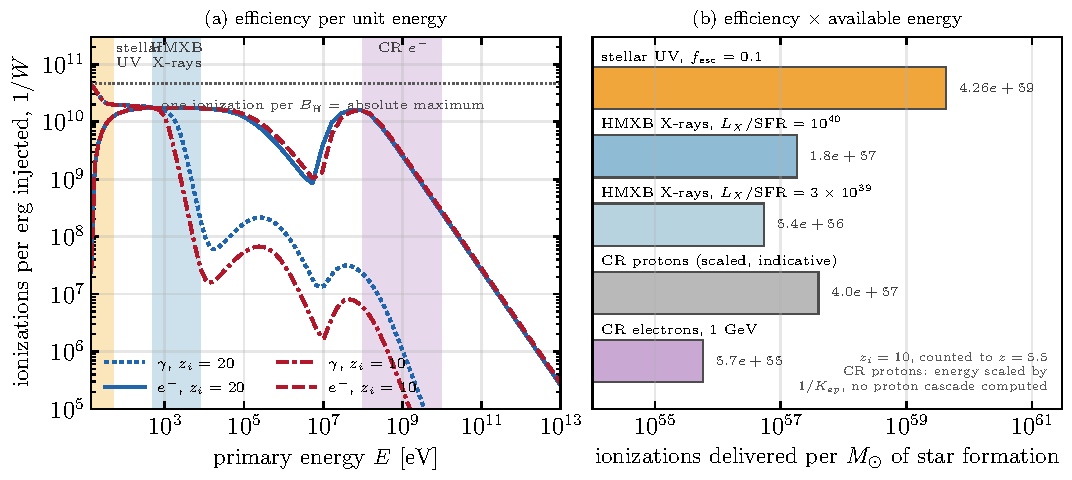
\includegraphics[width=\textwidth]{fig_reionization_budget.pdf}
  \caption{(a) Ionizations per erg of injected energy, $1/W(E)$, the quantity
  that actually matters for reionization, with the characteristic energies of
  the three source classes shaded. The dotted line is the absolute maximum,
  one ionization per $B_{\rm H}$; a threshold UV photon sits within a factor
  $1.5$ of it and nothing else comes close. (b) The same efficiency multiplied
  by the energy budget of each channel, per solar mass of star formation
  (Table~\ref{tab:budget}). The cosmic-ray proton bar is indicative only (no
  proton cascade was computed; see the flag on Table~\ref{tab:budget}).}
  \label{fig:budget}
\end{figure}

\paragraph{Confidence flags for this section.}
The $1/W$ column of Table~\ref{tab:pererg} inherits the $0.5\%$ numerical
uncertainty of Sect.~\ref{sec:verif}\,G and, above
\SI{37}{\mega\electronvolt}, the one-sided systematic of the omitted channels.
The energy budgets in Table~\ref{tab:budget} carry factor-of-a-few
uncertainties, dominated by $f_{\rm esc}$, $\langle E_\gamma\rangle$ and
$L_X/{\rm SFR}$; the cosmic-ray rows are the best constrained of the three,
since they are measured (Eq.~\ref{eq:crbudget}) rather than assumed; \emph{these are the reason no
result here is quoted to better than one significant figure}. The cosmic-ray
proton entry is not a calculation and is flagged as such. The conclusion is
robust to all of them, because it rests on a margin of $10^{2}$--$10^{4}$, not
on the precision of any single input.

%======================================================================
\section*{Reproducibility}
%======================================================================
\begin{itemize}\itemsep1pt
\item \texttt{Notebooks/redo/stage8\_photon\_yield.py} --- builds\\
      \texttt{redo\_photon\_yield\_table.npz} (\SI{181}{\second}).
      Parameters: $N_{\rm path}=192$, $N_s=64$, 120 energy nodes
      (\SIrange{13.61}{1e13}{\electronvolt}), 22 redshift rows
      ($3.0\le z\le20.0$), $x_e=10^{-4}$, $z_{\rm final}=5.5$
      (\texttt{Ne}) and $3.0$ (\texttt{Nt}).
\item \texttt{Notebooks/redo/stage8\_verify.py} $\to$
      \texttt{stage8\_verify.log} --- all checks of Sect.~\ref{sec:verif}.
\item \texttt{Notebooks/redo/stage8\_converge.py} $\to$
      \texttt{stage8\_converge.log} --- the doubled-resolution run.
\item \texttt{Notebooks/redo/stage8\_figure.py} $\to$\\
      \texttt{manuscript/figures\_redo/}\\
      \texttt{fig\_ionizations\_per\_primary.\{pdf,png\}}.
\item Electron input: \texttt{redo\_cascade\_table.npz} from
      \texttt{stage2\_cascade.py} (unchanged).
\item \texttt{Notebooks/redo/stage9\_budget.py} $\to$
      \texttt{stage9\_budget.log} --- Sect.~\ref{sec:why}, all budget numbers.
\item \texttt{Notebooks/redo/stage9\_verify\_budget.py} $\to$
      \texttt{stage9\_verify\_budget.log} --- provenance of the cosmic-ray
      budget: the Milky Way anchor, the IMF factor recomputed from
      \citet{chabrier03} and \citet{salpeter55}, and the agreement between
      the two routes.
\item \texttt{Notebooks/redo/stage9\_figure.py} $\to$\\
      \texttt{manuscript/figures\_redo/fig\_reionization\_budget.\{pdf,png\}}.
\item No stochastic method is used anywhere, so no random seed is involved.
\end{itemize}

%======================================================================
\begin{thebibliography}{99}
\bibitem[Blumenthal \& Gould(1970)]{blumenthal70}
  Blumenthal, G.~R., \& Gould, R.~J. 1970, Rev.\ Mod.\ Phys., 42, 237.
\bibitem[Breit \& Wheeler(1934)]{breit34}
  Breit, G., \& Wheeler, J.~A. 1934, Phys.\ Rev., 46, 1087.
\bibitem[Furlanetto \& Stoever(2010)]{furlanetto10}
  Furlanetto, S.~R., \& Stoever, S.~J. 2010, MNRAS, 404, 1869.
\bibitem[Gould(1972)]{gould72}
  Gould, R.~J. 1972, Physica, 60, 145.
\bibitem[Heitler(1954)]{heitler54}
  Heitler, W. 1954, The Quantum Theory of Radiation, 3rd ed. (Oxford: Clarendon),
  \S22 and \S26.
\bibitem[Jauch \& Rohrlich(1976)]{jauch76}
  Jauch, J.~M., \& Rohrlich, F. 1976, The Theory of Photons and Electrons,
  2nd ed. (Berlin: Springer), \S11-3.
\bibitem[Karzas \& Latter(1961)]{karzas61}
  Karzas, W.~J., \& Latter, R. 1961, ApJS, 6, 167.
\bibitem[Kim et al.(2000)]{kim00}
  Kim, Y.-K., Santos, J.~P., \& Parente, F. 2000, Phys.\ Rev.\ A, 62, 052710.
\bibitem[Klein \& Nishina(1929)]{klein29}
  Klein, O., \& Nishina, Y. 1929, Z.\ Phys., 52, 853.
\bibitem[Motz et al.(1969)]{motz69}
  Motz, J.~W., Olsen, H.~A., \& Koch, H.~W. 1969, Rev.\ Mod.\ Phys., 41, 581.
\bibitem[Planck Collaboration(2020)]{planck18}
  Planck Collaboration 2020, A\&A, 641, A6.
\bibitem[Rybicki \& Lightman(1979)]{rl79}
  Rybicki, G.~B., \& Lightman, A.~P. 1979, Radiative Processes in Astrophysics
  (New York: Wiley), \S7.1, Eq.~(7.5).
\bibitem[Shull \& van Steenberg(1985)]{shull85}
  Shull, J.~M., \& van Steenberg, M.~E. 1985, ApJ, 298, 268.
\bibitem[Stone \& Kim(2002)]{stone02}
  Stone, P.~M., Kim, Y.-K., \& Desclaux, J.~P. 2002, J.\ Res.\ NIST, 107, 327;
  Stone, P.~M., \& Kim, Y.-K. 2002, J.\ Phys.\ B, 35, 1675.
\bibitem[Bolton \& Haehnelt(2007)]{bolton07}
  Bolton, J.~S., \& Haehnelt, M.~G. 2007, MNRAS, 382, 325.
\bibitem[Bosman et al.(2022)]{bosman22}
  Bosman, S.~E.~I., Davies, F.~B., Becker, G.~D., et al. 2022, MNRAS, 514, 55.
\bibitem[Bouwens et al.(2016)]{bouwens16}
  Bouwens, R.~J., Smit, R., Labb\'e, I., et al. 2016, ApJ, 831, 176.
\bibitem[Chen \& Kamionkowski(2004)]{chen04}
  Chen, X., \& Kamionkowski, M. 2004, Phys.\ Rev.\ D, 70, 043502.
\bibitem[Finkelstein et al.(2019)]{finkelstein19}
  Finkelstein, S.~L., D'Aloisio, A., Paardekooper, J.-P., et al. 2019, ApJ, 879, 36.
\bibitem[Fragos et al.(2013)]{fragos13}
  Fragos, T., Lehmer, B.~D., Naoz, S., Zezas, A., \& Basu-Zych, A. 2013,
  ApJ, 776, L31.
\bibitem[Kennicutt(1998)]{kennicutt98}
  Kennicutt, R.~C. 1998, ARA\&A, 36, 189.
\bibitem[Lehmer et al.(2021)]{lehmer21}
  Lehmer, B.~D., Eufrasio, R.~T., Basu-Zych, A., et al. 2021, ApJ, 907, 17.
\bibitem[Leite et al.(2017)]{leite17}
  Leite, N., Evoli, C., D'Angelo, M., et al. 2017, MNRAS, 469, 416.
\bibitem[Madau \& Dickinson(2014)]{madau14}
  Madau, P., \& Dickinson, M. 2014, ARA\&A, 52, 415.
\bibitem[McQuinn(2012)]{mcquinn12}
  McQuinn, M. 2012, MNRAS, 426, 1349.
\bibitem[Merten et al.(2017)]{merten17}
  Merten, L., Becker Tjus, J., Eichmann, B., \& Dettmar, R.-J. 2017,
  Astropart.\ Phys., 90, 75.
\bibitem[Mesinger et al.(2013)]{mesinger13}
  Mesinger, A., Ferrara, A., \& Spiegel, D.~S. 2013, MNRAS, 431, 621.
\bibitem[Mineo et al.(2012)]{mineo12}
  Mineo, S., Gilfanov, M., \& Sunyaev, R. 2012, MNRAS, 419, 2095.
\bibitem[Oh(2001)]{oh01}
  Oh, S.~P. 2001, ApJ, 553, 499.
\bibitem[Robertson et al.(2015)]{robertson15}
  Robertson, B.~E., Ellis, R.~S., Furlanetto, S.~R., \& Dunlop, J.~S. 2015,
  ApJ, 802, L19.
\bibitem[Sazonov \& Sunyaev(2015)]{sazonov15}
  Sazonov, S., \& Sunyaev, R. 2015, MNRAS, 454, 3464.
\bibitem[Valdes \& Ferrara(2008)]{valdes08}
  Vald\'es, M., \& Ferrara, A. 2008, MNRAS, 387, L8.
\bibitem[Venkatesan et al.(2001)]{venkatesan01}
  Venkatesan, A., Giroux, M.~L., \& Shull, J.~M. 2001, ApJ, 563, 1.
\bibitem[Caprioli \& Spitkovsky(2014)]{caprioli14}
  Caprioli, D., \& Spitkovsky, A. 2014, ApJ, 783, 91.
\bibitem[Chabrier(2003)]{chabrier03}
  Chabrier, G. 2003, PASP, 115, 763.
\bibitem[Drury et al.(1989)]{drury89}
  Drury, L.~O'C., Markiewicz, W.~J., \& V\"olk, H.~J. 1989, A\&A, 225, 179.
\bibitem[Gessey-Jones et al.(2023)]{gesseyjones23}
  Gessey-Jones, T., Fialkov, A., de Lera Acedo, E., Handley, W.~J., \&
  Barkana, R. 2023, MNRAS, 526, 4262.
\bibitem[Licquia \& Newman(2015)]{licquia15}
  Licquia, T.~C., \& Newman, J.~A. 2015, ApJ, 806, 96.
\bibitem[Salpeter(1955)]{salpeter55}
  Salpeter, E.~E. 1955, ApJ, 121, 161.
\bibitem[Strong et al.(2010)]{strong10}
  Strong, A.~W., Porter, T.~A., Digel, S.~W., et al. 2010, ApJ, 722, L58.
\bibitem[Woosley \& Weaver(1995)]{woosley95}
  Woosley, S.~E., \& Weaver, T.~A. 1995, ApJS, 101, 181.
\bibitem[Zdziarski \& Svensson(1989)]{zdziarski89}
  Zdziarski, A.~A., \& Svensson, R. 1989, ApJ, 344, 551.
\end{thebibliography}

\end{document}
